%% LyX 1.3 created this file.  For more info, see http://www.lyx.org/.
%% Do not edit unless you really know what you are doing.
\documentclass[english, 12pt]{article}
\usepackage{times}
%\usepackage{algorithm2e}
\usepackage{url}
\usepackage{bbm}
\usepackage[T1]{fontenc}
\usepackage[latin1]{inputenc}
\usepackage{geometry}
\geometry{verbose,letterpaper,tmargin=2cm,bmargin=2cm,lmargin=1.5cm,rmargin=1.5cm}
\usepackage{rotating}
\usepackage{color}
\usepackage{graphicx}
\usepackage{amsmath, amsthm, amssymb}
\usepackage{setspace}
\usepackage{lineno}
\usepackage{hyperref}
\usepackage{bbm}
\usepackage{makecell}
\usepackage{placeins}
\usepackage{subcaption}

%\renewcommand{\arraystretch}{1.8}

%\linenumbers
%\doublespacing
\onehalfspacing
%\usepackage[authoryear]{natbib}
\usepackage{natbib} \bibpunct{(}{)}{;}{author-year}{}{,}

%Pour les rajouts
\usepackage{color}
\definecolor{trustcolor}{rgb}{0,0,1}

\usepackage{dsfont}
\usepackage[warn]{textcomp}
\usepackage{adjustbox}
\usepackage{multirow}
\usepackage{subcaption}
\usepackage{graphicx}
\graphicspath{{../figures/}}
\DeclareMathOperator*{\argmin}{\arg\!\min}

\let\tabbeg\tabular
\let\tabend\endtabular
\renewenvironment{tabular}{\begin{adjustbox}{max width=0.95\textwidth}\tabbeg}{\tabend\end{adjustbox}}

\makeatletter

%%%%%%%%%%%%%%%%%%%%%%%%%%%%%% LyX specific LaTeX commands.
%% Bold symbol macro for standard LaTeX users
%\newcommand{\boldsymbol}[1]{\mbox{\boldmath $#1$}}

%% Because html converters don't know tabularnewline
\providecommand{\tabularnewline}{\\}
\renewcommand*{\arraystretch}{1.2}

\usepackage{babel}
\makeatother


\begin{document}

\renewcommand{\thefigure}{S\arabic{figure}}
\setcounter{figure}{0}
\renewcommand{\thetable}{S\arabic{table}}
\setcounter{table}{0}
\renewcommand{\theequation}{S\arabic{equation}}
\setcounter{equation}{0}

\section*{Supplementary Tables and Figures}

\vspace{5em}

%%%%%%%%%%%%%%%%%%%%%%%%%%%%%%%%%%%%%%%%%%%%%%%%%%%%%%%%%%%%%%%%%%%%%%%%%%%%%%%%



\begin{figure}[h]
	\centering
	\includegraphics[width=0.9\textwidth]{lasso-ancestry-geno}
	\caption{Partial correlation (and 95\% CI) in the UK test set versus in a test set from another ancestry group. Each point represents a phenotype (only 83 of the continuous phenotypes here) and training has been performed with penalized regression on UK individuals (training 1 in table 1) and \textbf{genotyped} variants. The slope (in blue) is computed using Deming regression accounting for standard errors in both x and y.
	This slope (squared) is provided in the title, which we report as the relative predictive performance compared to testing in UK.}
	\label{fig:lasso-ancestry-geno}
\end{figure}

\begin{figure}[h]
\centering
\includegraphics[width=0.9\textwidth]{ldpred2-ancestry}
\caption{Partial correlation (and 95\% CI) in the UK test set versus in a test set from another ancestry group. Each point represents a phenotype and training has been performed with \textbf{LDpred2-auto} on UK individuals (training 1 in table 1) and HapMap3 variants. The slope (in blue) is computed using Deming regression accounting for standard errors in both x and y.
This slope (squared) is provided in the title, which we report as the relative predictive performance compared to testing in UK.}
\label{fig:ldpred2-ancestry}
\end{figure}

%%%%%%%%%%%%%%%%%%%%%%%%%%%%%%%%%%%%%%%%%%%%%%%%%%%%%%%%%%%%%%%%%%%%%%%%%%%%%%%%

\begin{figure}[htbp]
	\centerline{\includegraphics[width=0.85\textwidth]{ratio-dist-restricted}}
	\caption{Relative predictive performance with UK compared to PC distance with UK. PCA is computed using individuals from test 1 (Table 1), and PC distances are computed using Euclidean distance between geometric medians of the first 32 PC scores of each ancestry group (shown in figure \ref{fig:PCs-restricted}). Relative performance values are the ones reported in figure 1 of the main text.}
	\label{fig:ratio-dist2}
\end{figure}

\begin{figure}[htbp]
\centerline{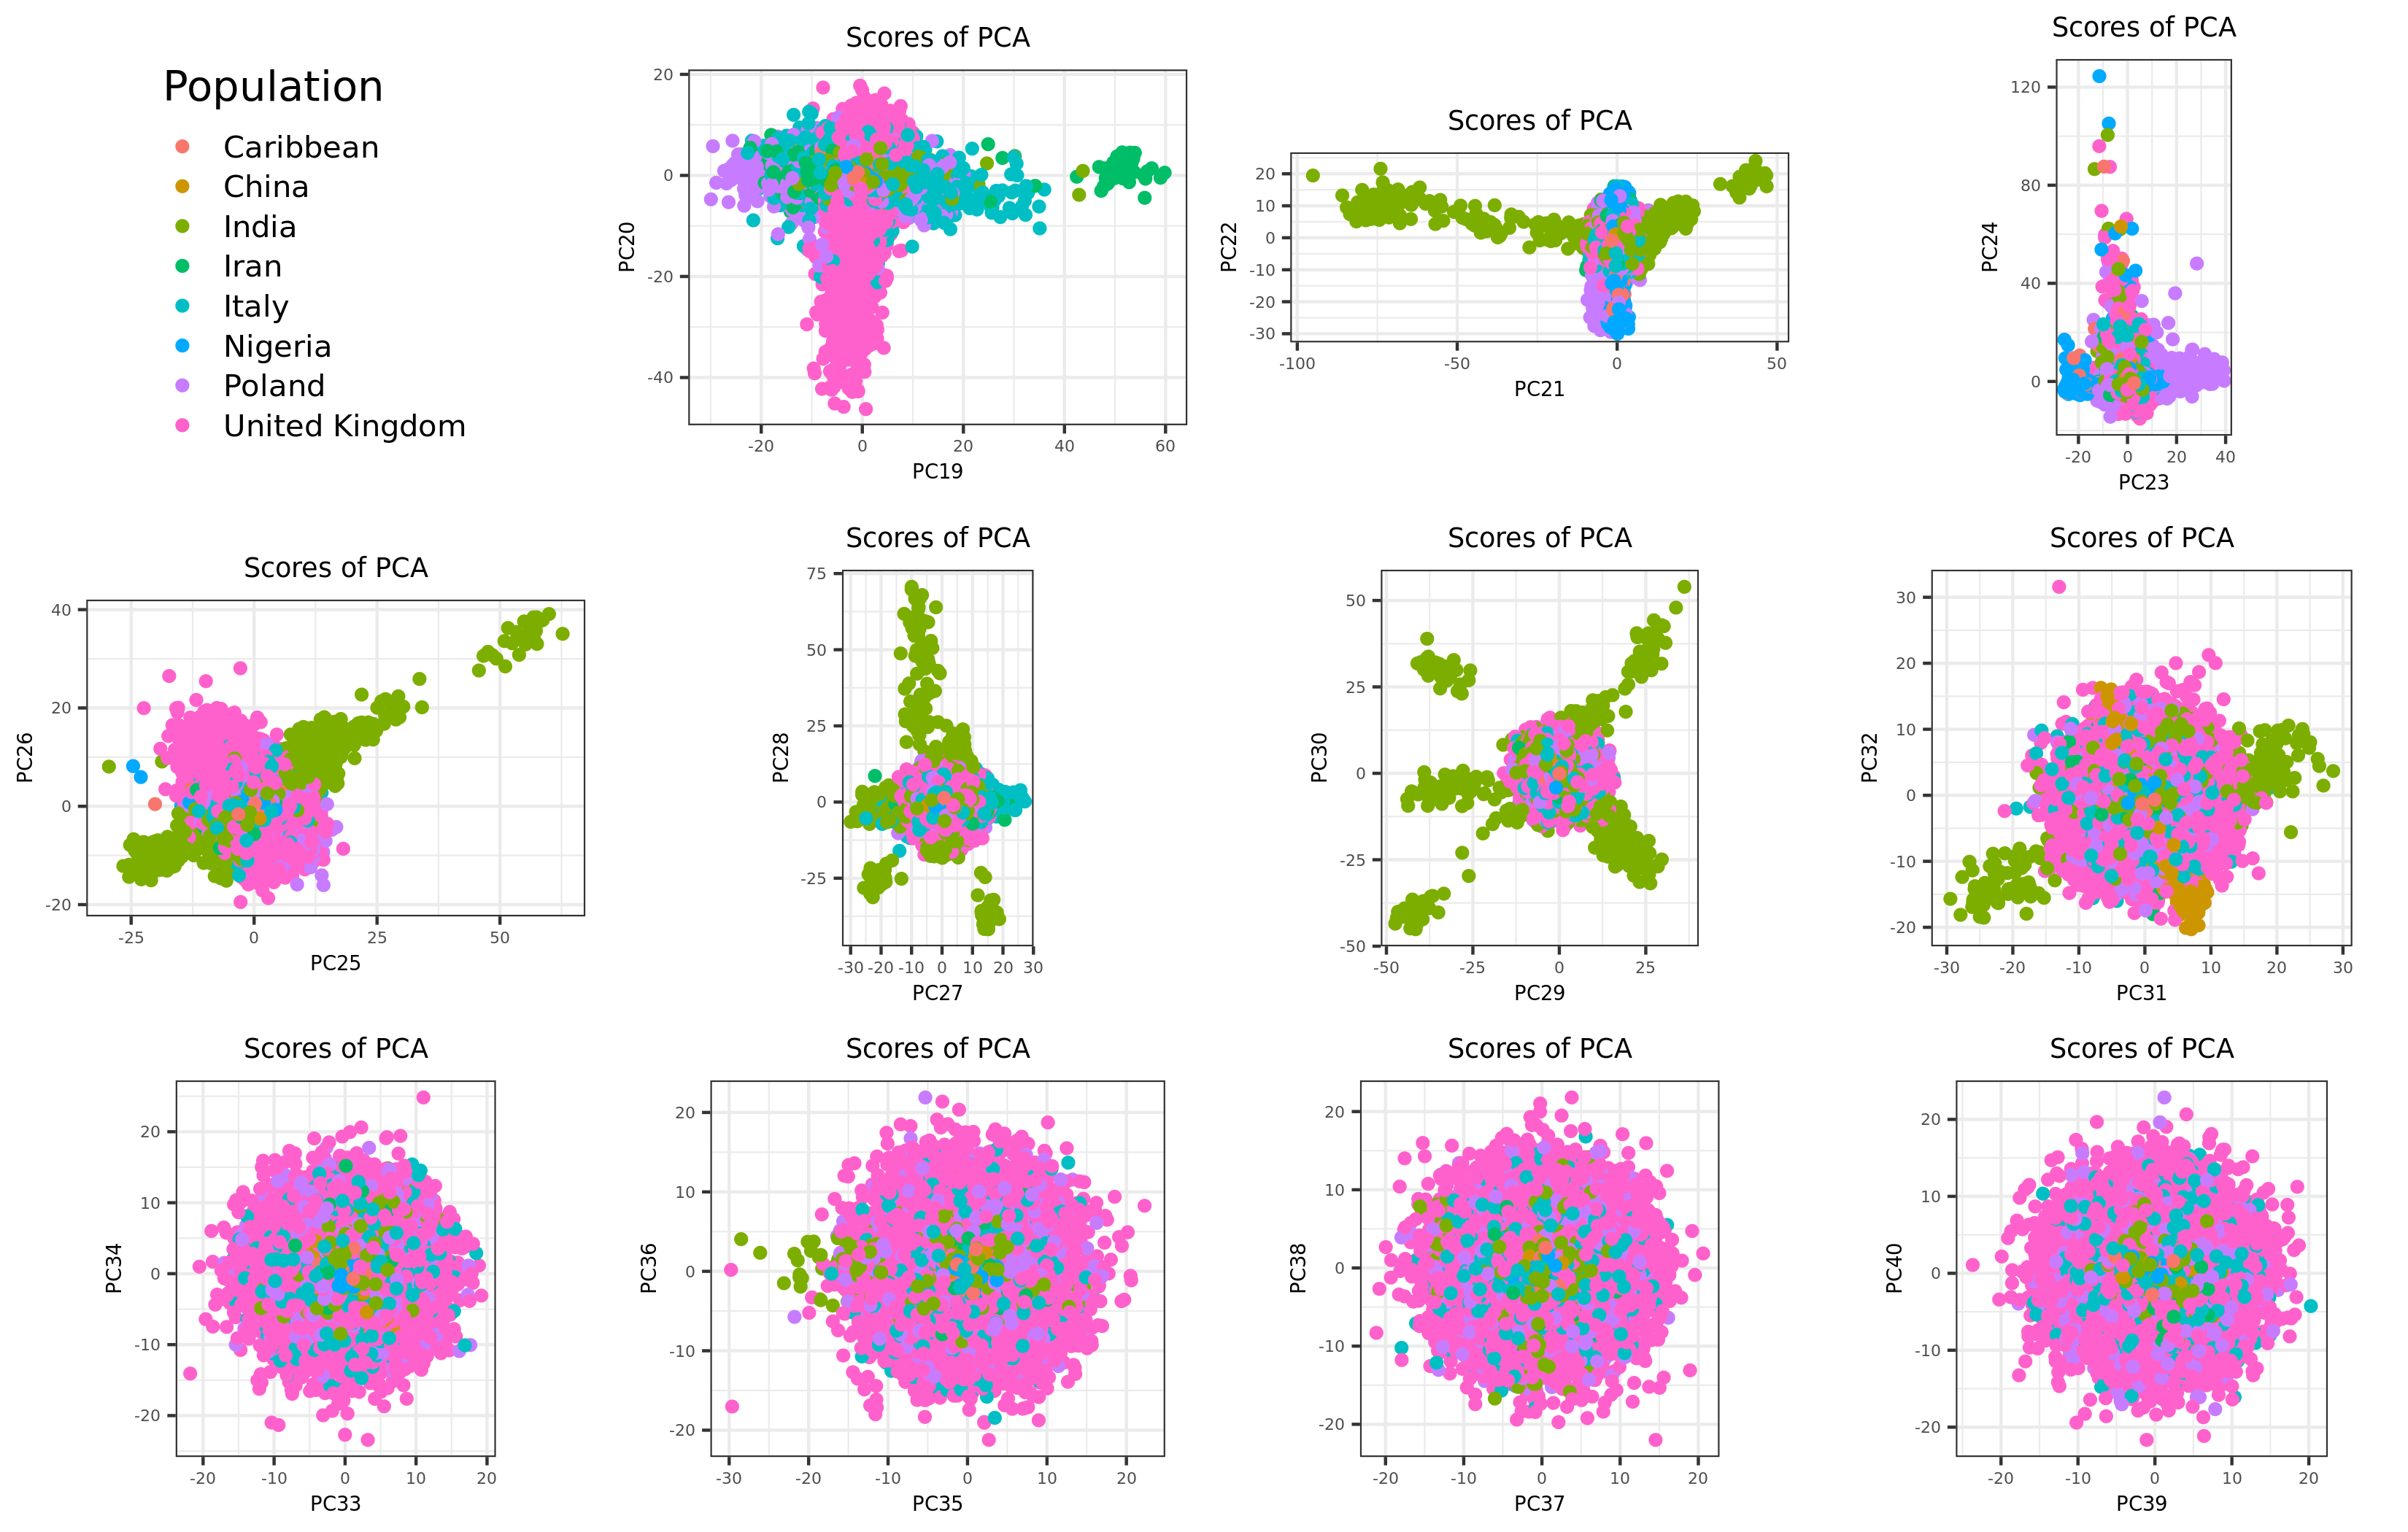
\includegraphics[width=0.95\textwidth]{PC-scores-restricted}}
\caption{PC scores 19 to 40 when PCA is computed using individuals from test 1 (Table 1). First 32 PCs visually capture some population structure.}
\label{fig:PCs-restricted}	
\end{figure}

%%%%%%%%%%%%%%%%%%%%%%%%%%%%%%%%%%%%%%%%%%%%%%%%%%%%%%%%%%%%%%%%%%%%%%%%%%%%%%%%

\begin{figure}[h]
	\centering
	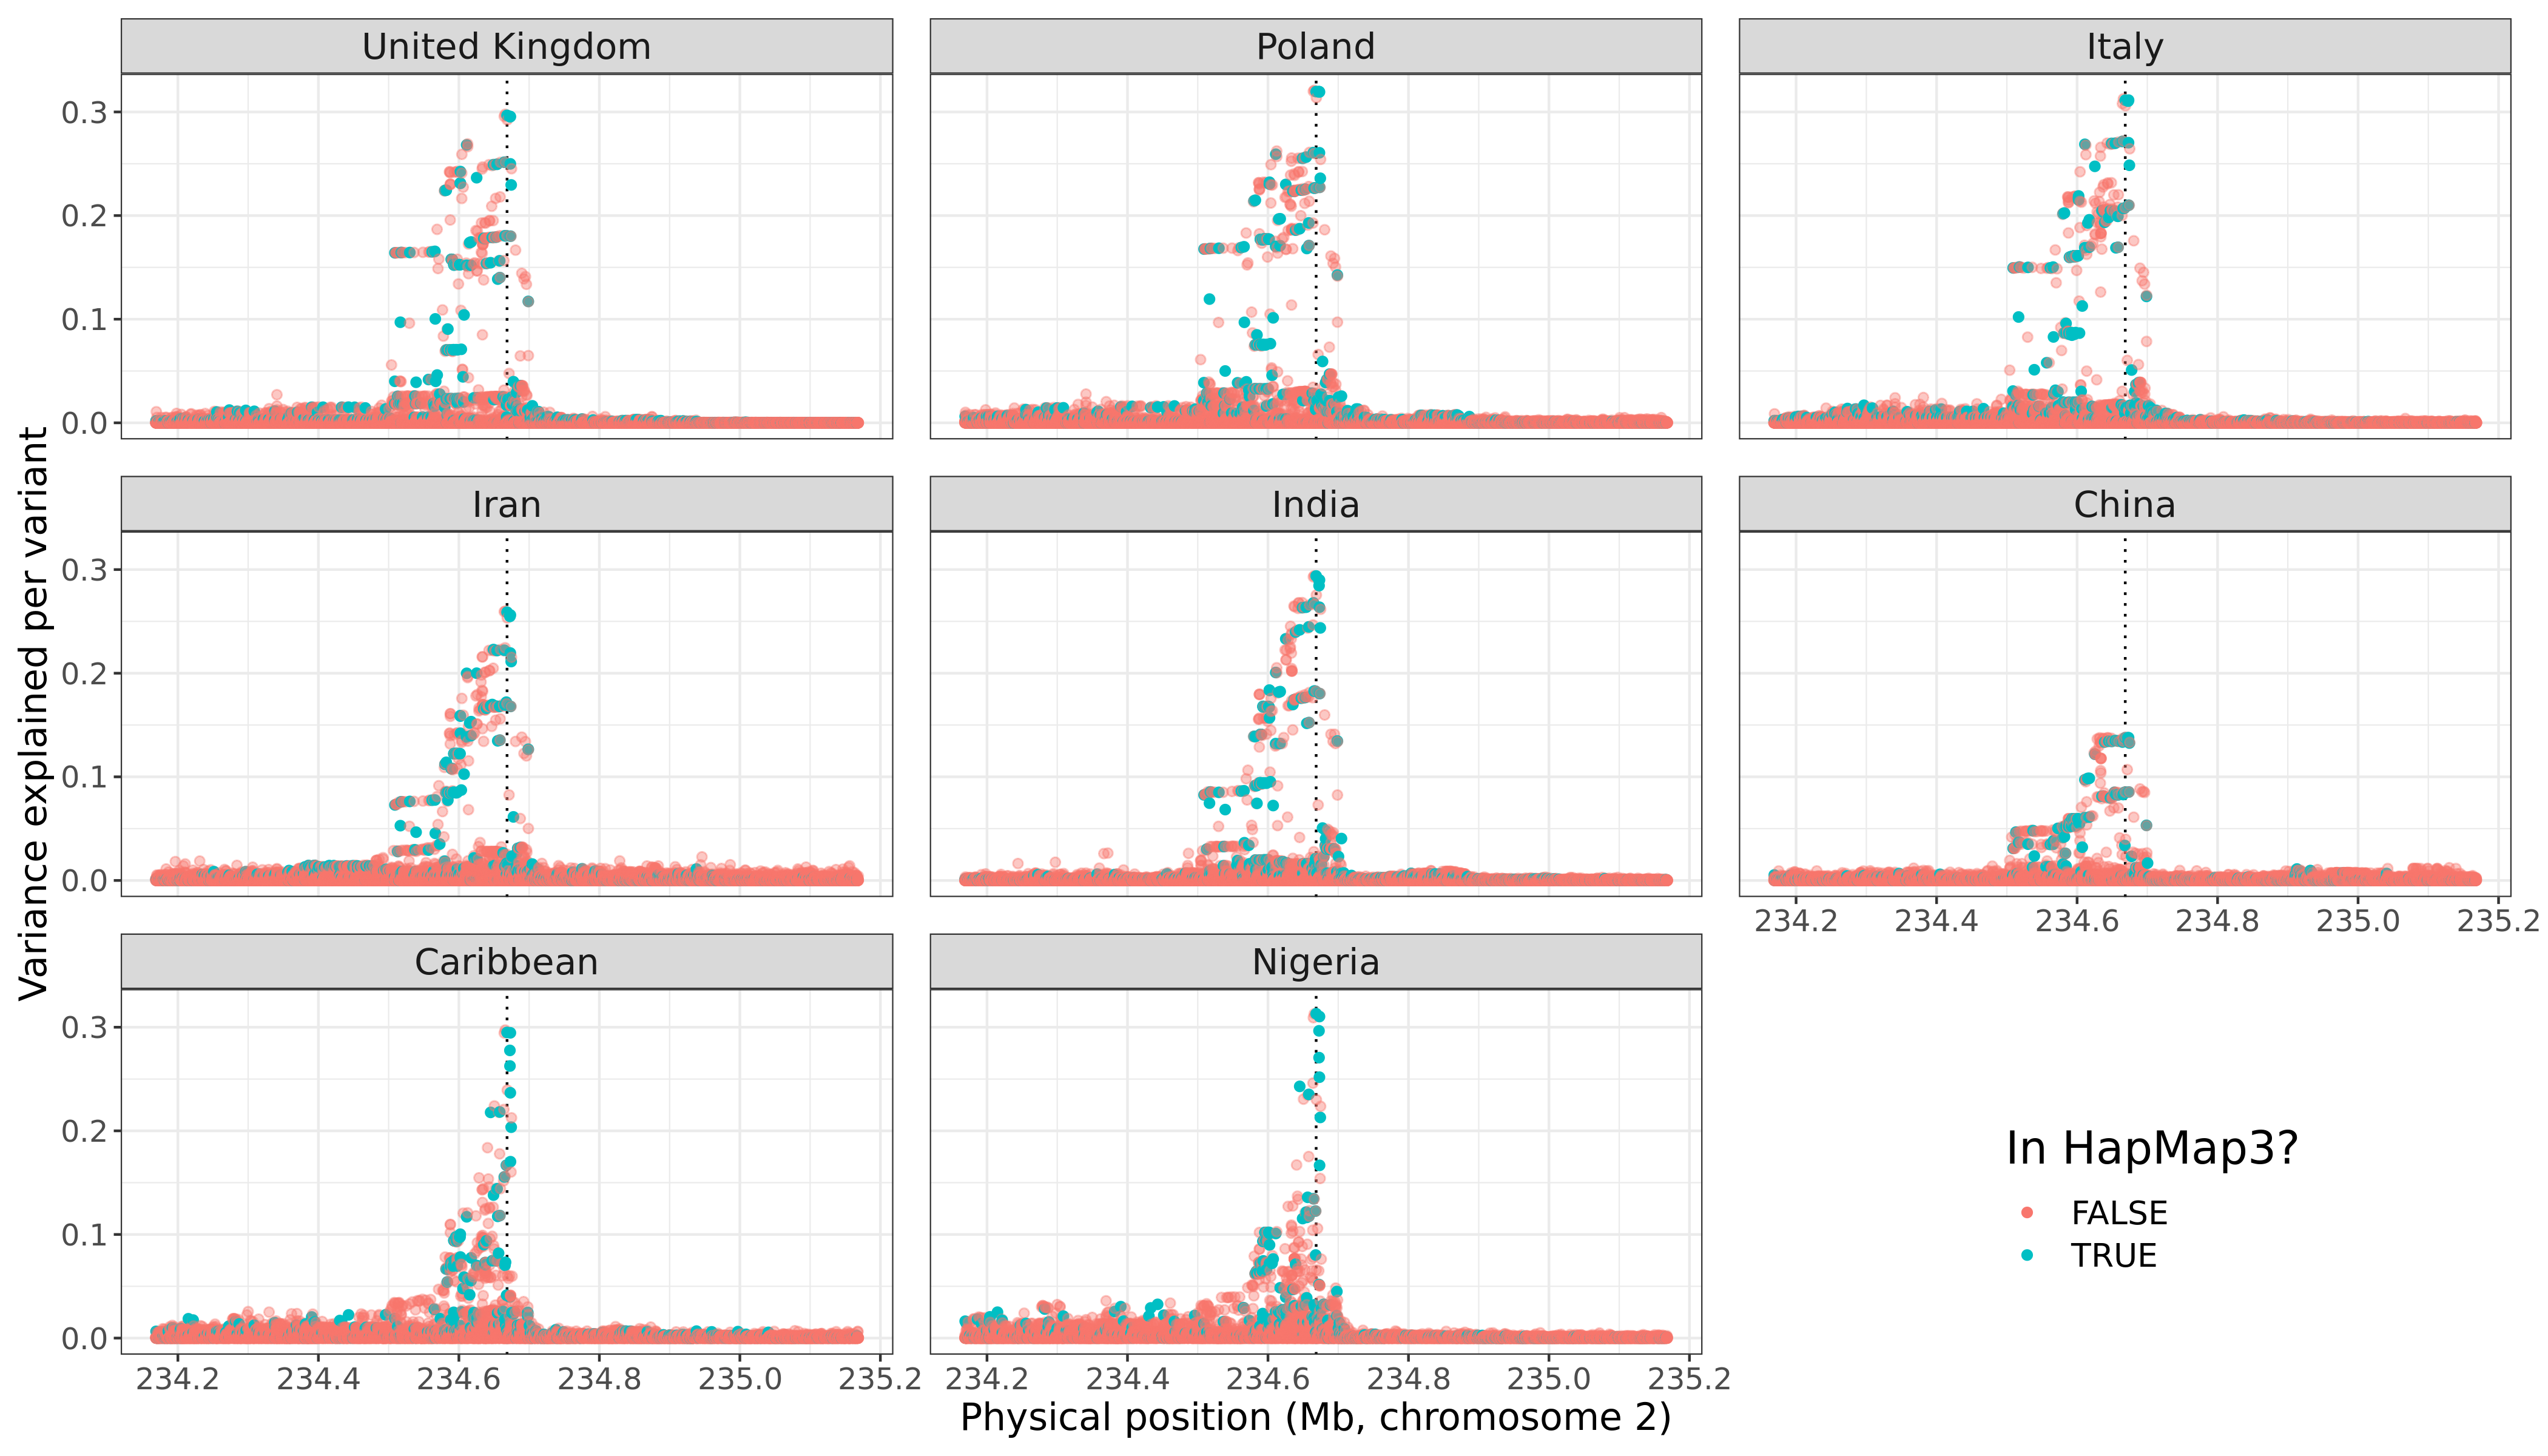
\includegraphics[width=0.9\textwidth]{zoom_log_bilirubin}
	\caption{Zoomed Manhattan plot for total \textbf{bilirubin} concentration. Here the (partial) correlation $r$ between each variant and the phenotype is reported, where $r = t / \sqrt{n + t^2}$, where $t$ is the t-score and $n$ is the degrees of freedom (the sample size minus the number of variables in the model, i.e.\ the covariates used in the GWAS, the intercept and the variant).The GWAS includes all variants with an imputation INFO score larger than 0.3 and within a 500Kb radius around the top hit from the GWAS performed in the UK training set and on the HapMap3 variants, represented by a vertical dotted line.}
	\label{fig:zoom-bilirubin}
\end{figure}

\begin{figure}[h]
	\centering
	\includegraphics[width=0.9\textwidth]{top3_log_bilirubin}
	\caption{Effect sizes and variance explained for the top three variants from figure \ref{fig:zoom-bilirubin}.}
	\label{fig:top3-bilirubin}
\end{figure}

\begin{figure}[h]
	\centering
	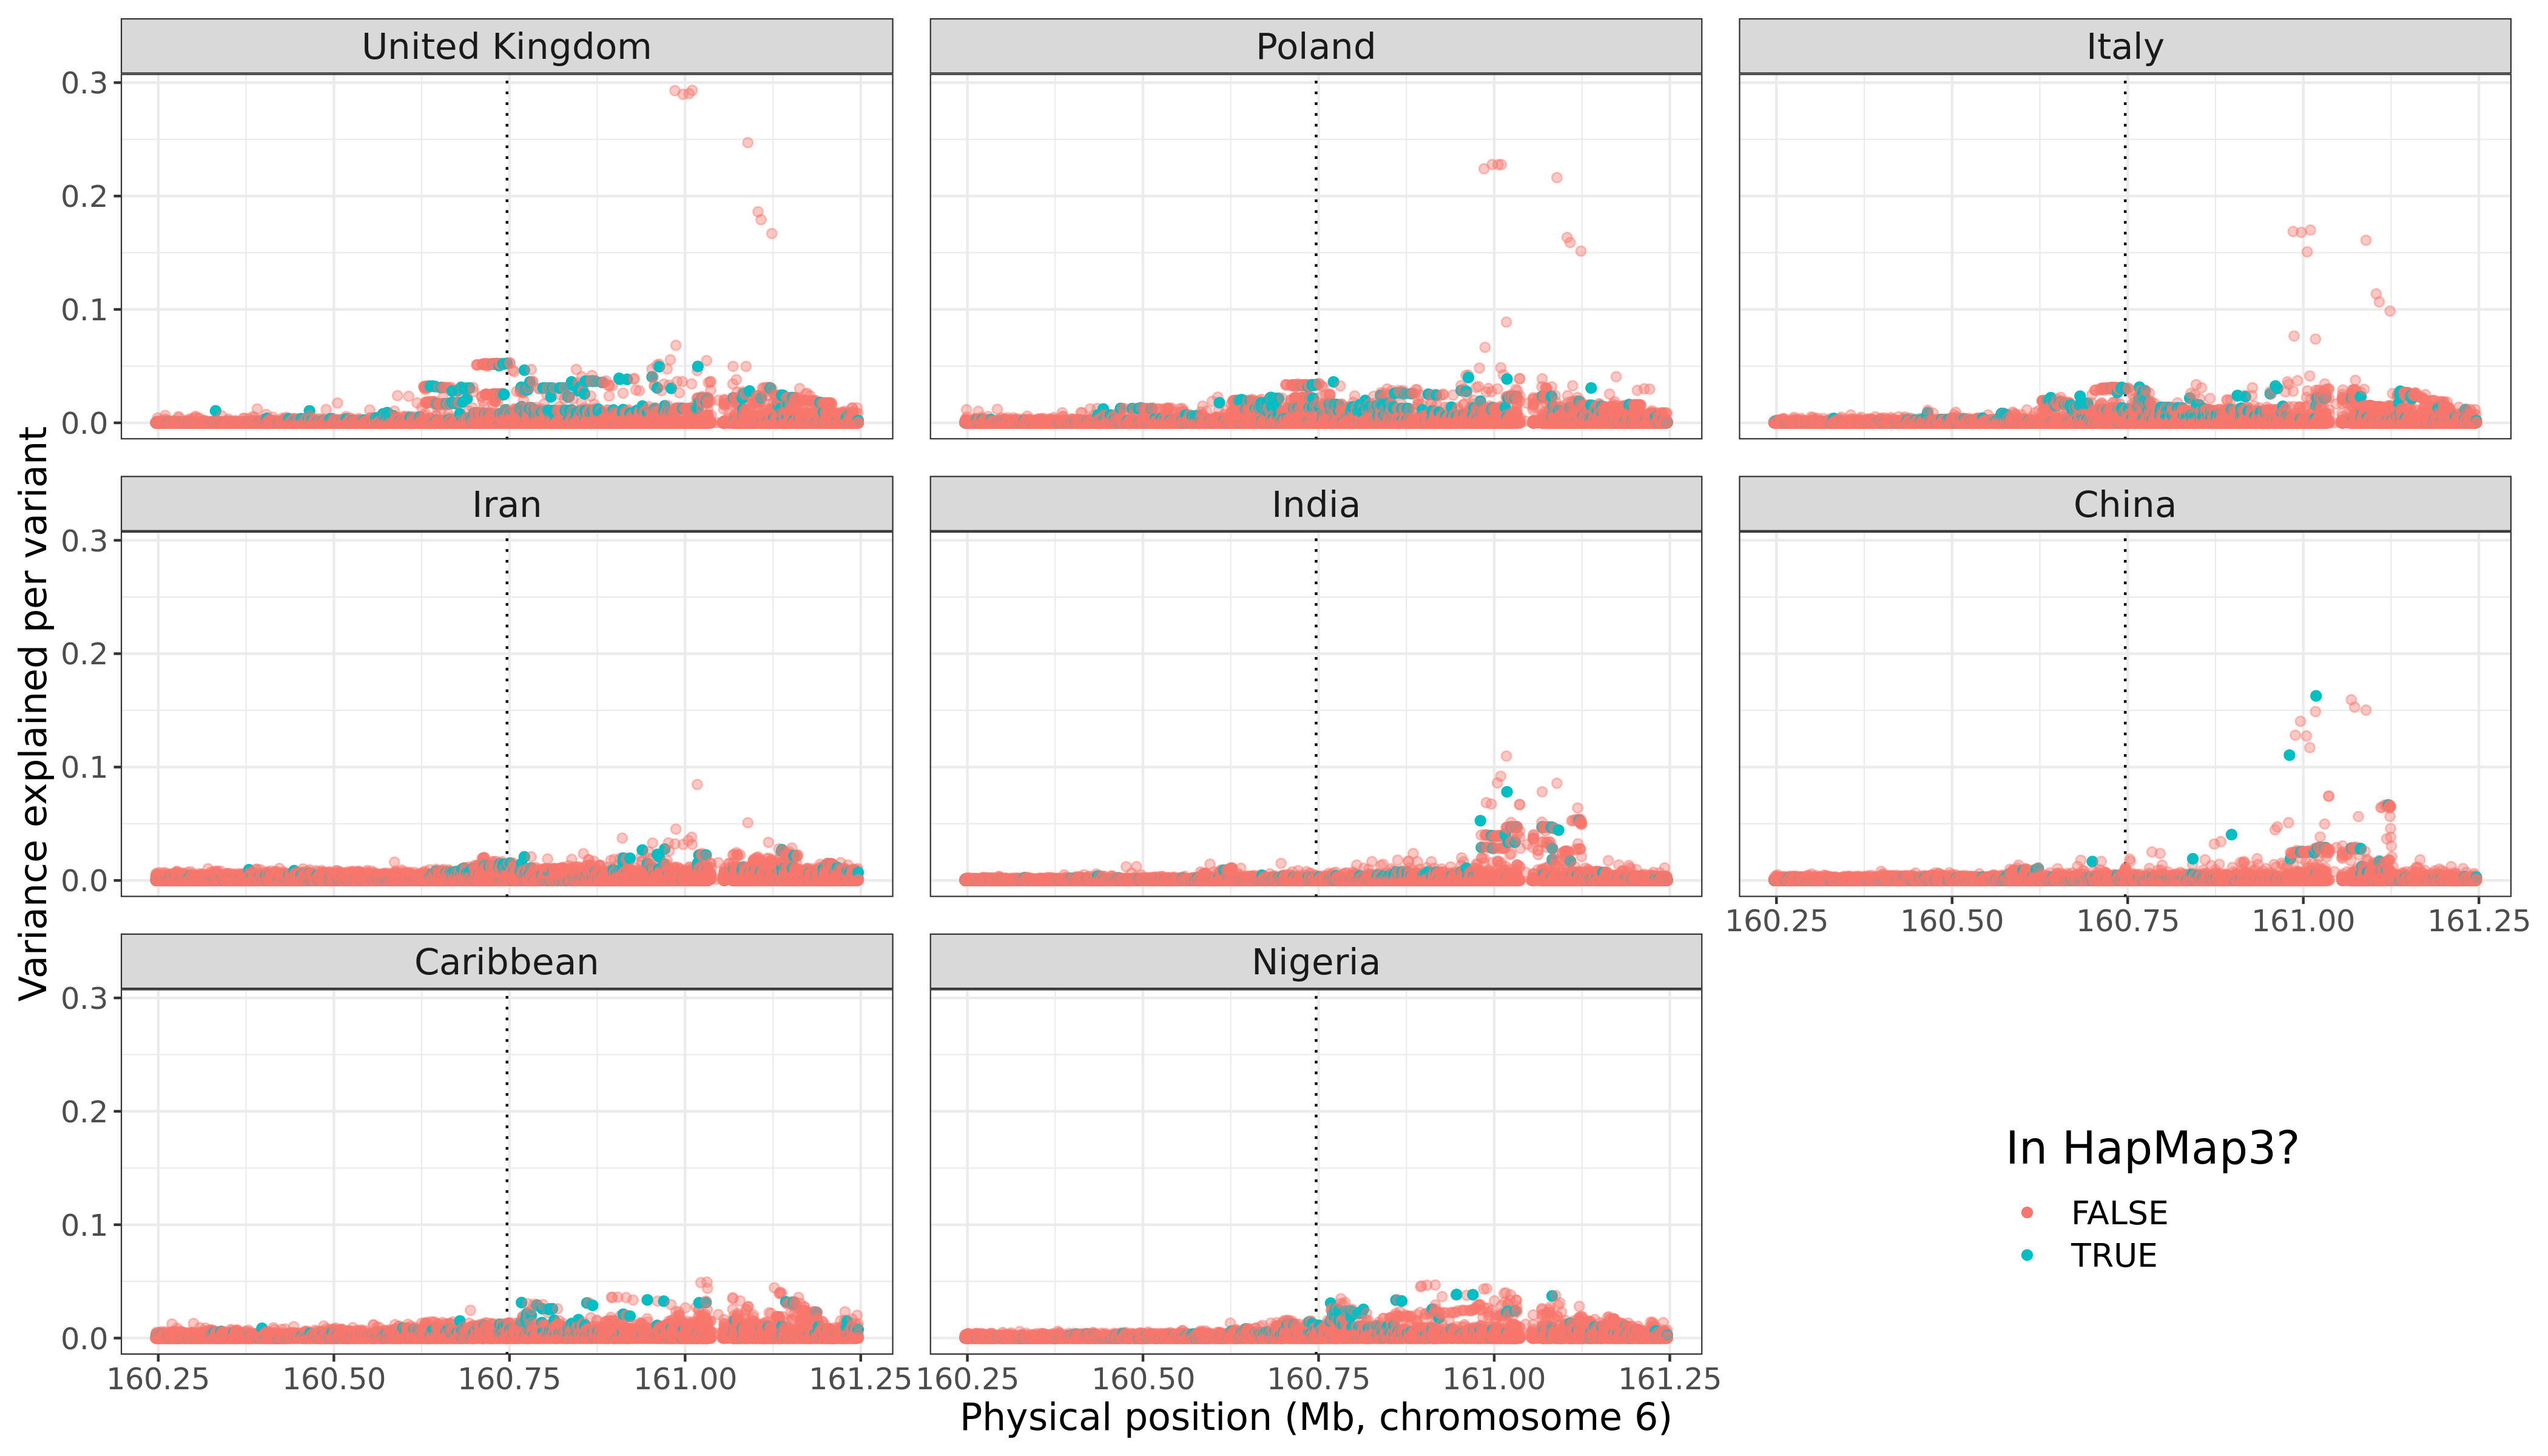
\includegraphics[width=0.9\textwidth]{zoom_log_lipoA}
	\caption{Zoomed Manhattan plot for \textbf{lipoprotein A} concentration. Here the (partial) correlation $r$ between each variant and the phenotype is reported, where $r = t / \sqrt{n + t^2}$, where $t$ is the t-score and $n$ is the degrees of freedom (the sample size minus the number of variables in the model, i.e.\ the covariates used in the GWAS, the intercept and the variant). The GWAS includes all variants with an imputation INFO score larger than 0.3 and within a 500Kb radius around the top hit from the GWAS performed in the UK training set and on the HapMap3 variants, represented by a vertical dotted line.}
	\label{fig:zoom-lipoA}
\end{figure}

\begin{figure}[h]
	\centering
	\includegraphics[width=0.9\textwidth]{top3_log_lipoA}
	\caption{Effect sizes and variance explained for the top three variants from figure \ref{fig:zoom-lipoA}.}
	\label{fig:top3-lipoA}
\end{figure}

\begin{figure}[h]
	\centering
	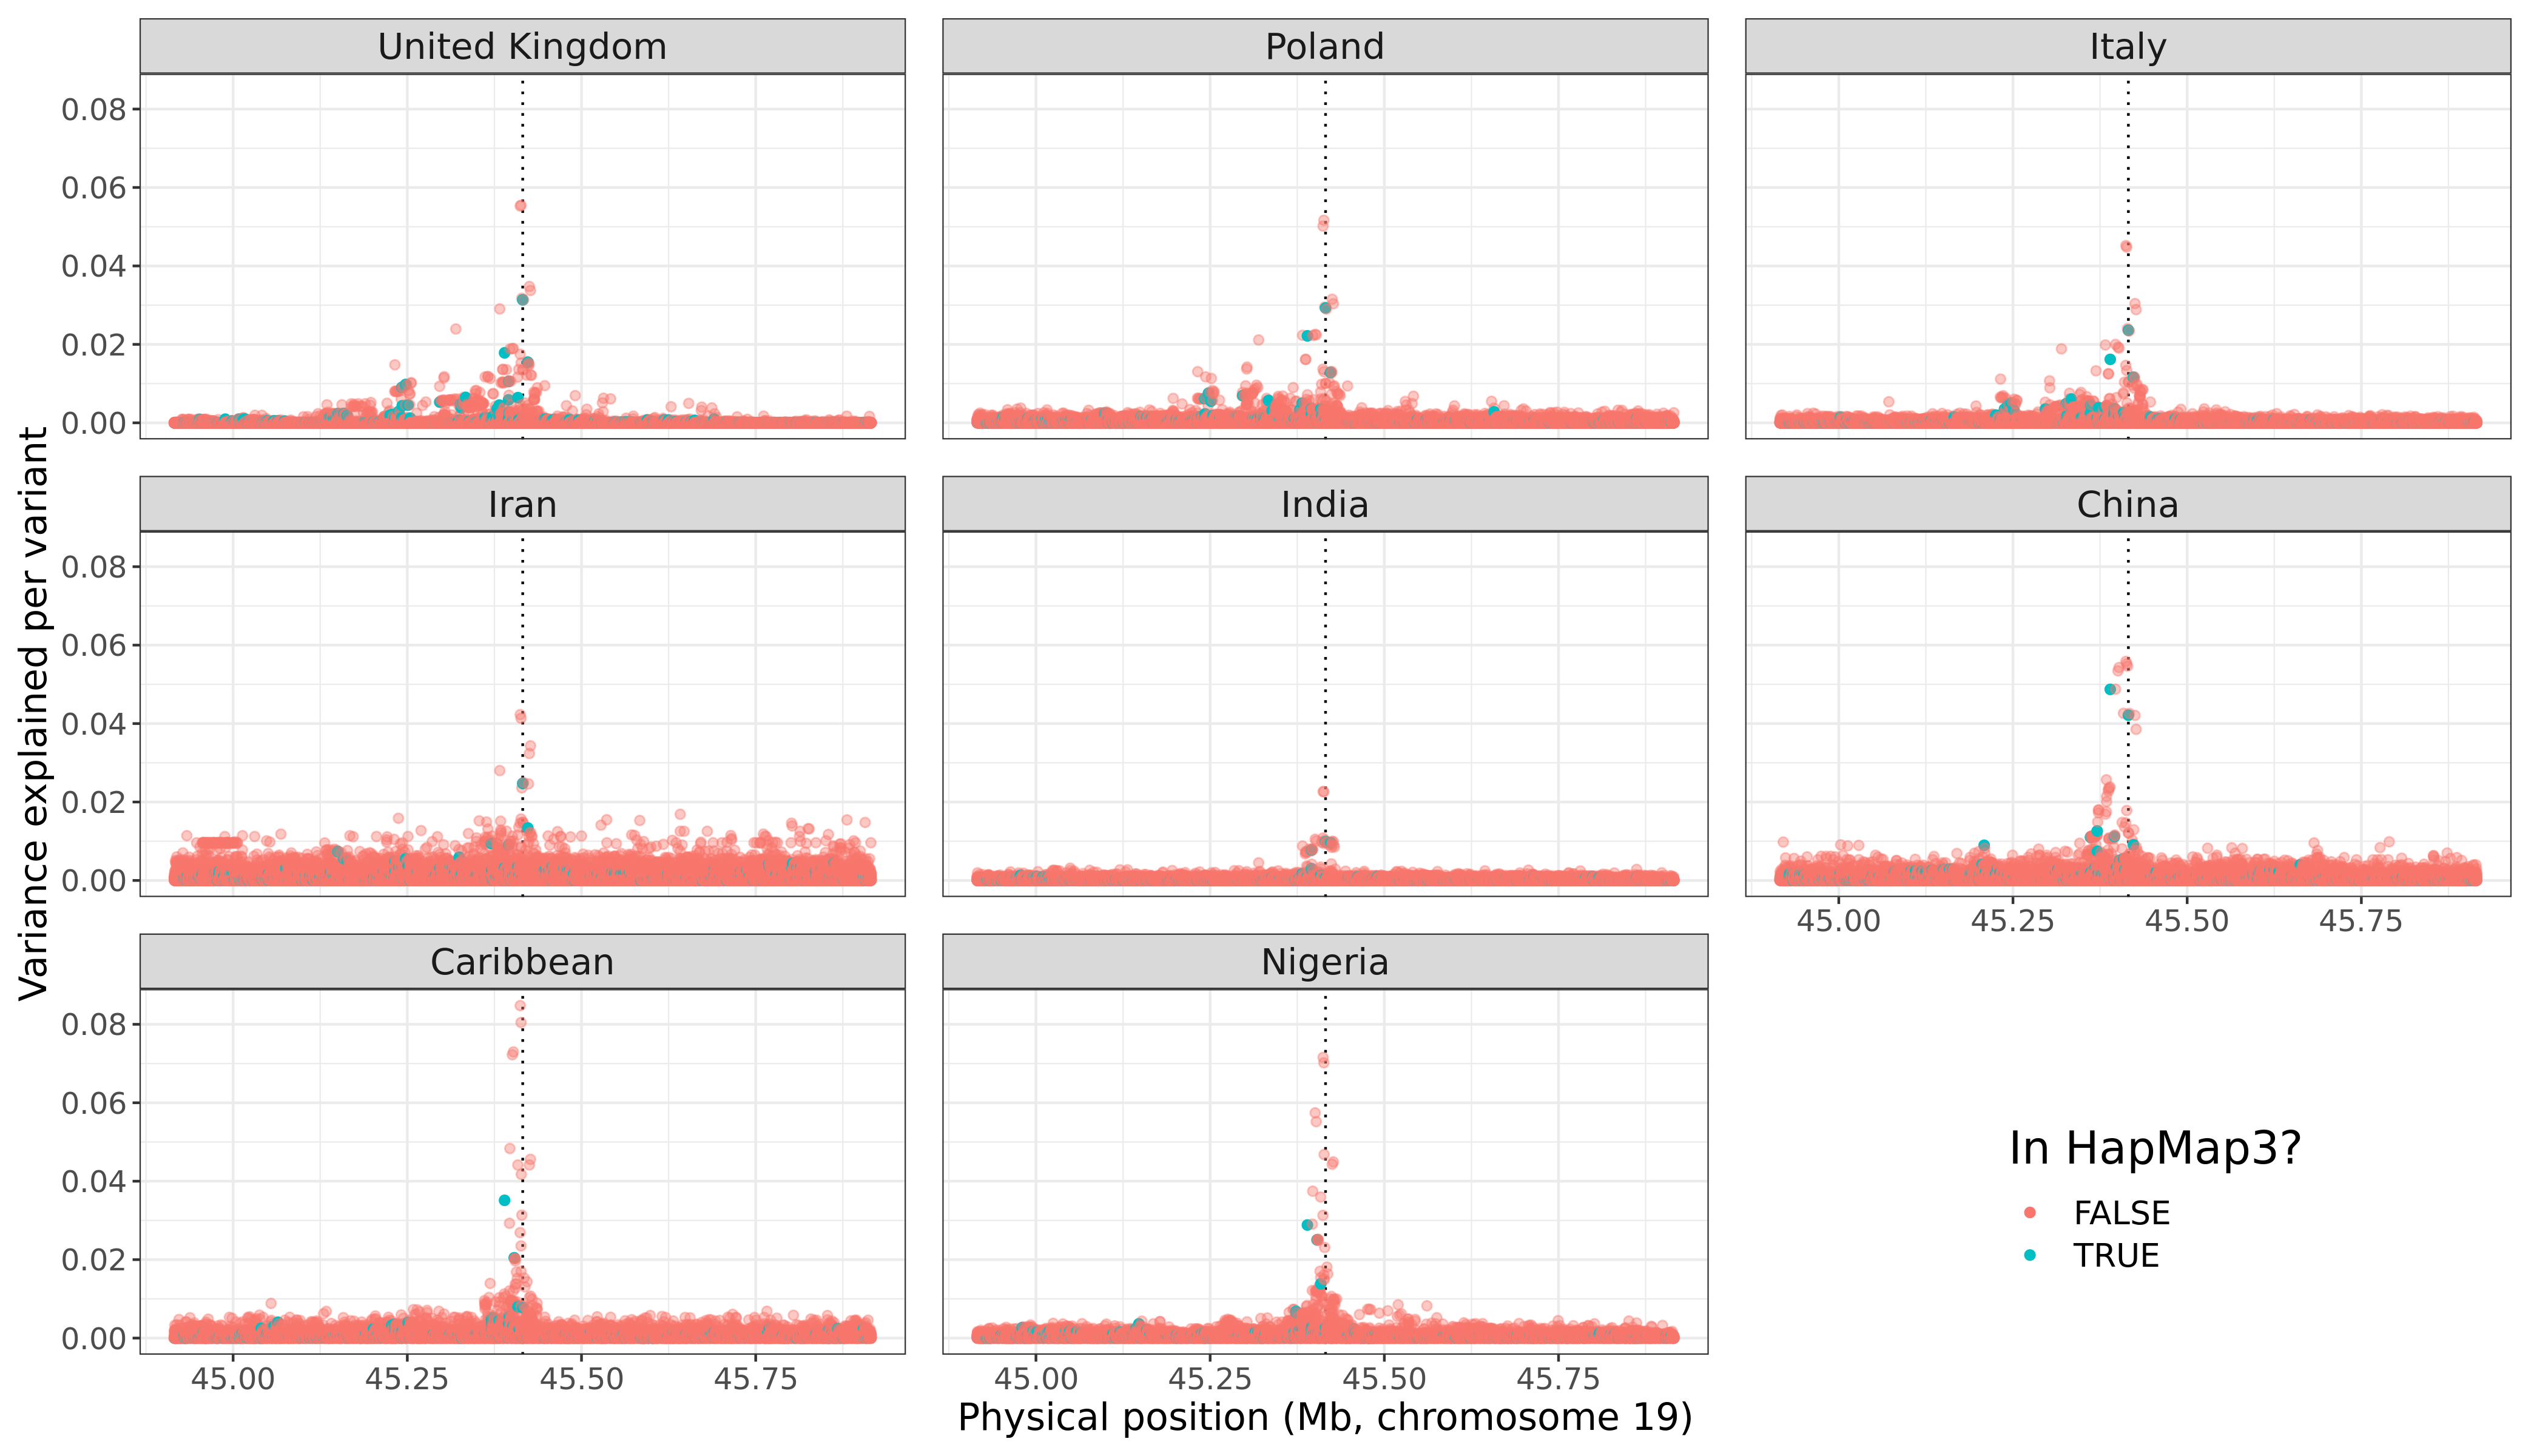
\includegraphics[width=0.9\textwidth]{zoom_apoB}
	\caption{Zoomed Manhattan plot for \textbf{apolipoprotein B} concentration. Here the (partial) correlation $r$ between each variant and the phenotype is reported, where $r = t / \sqrt{n + t^2}$, where $t$ is the t-score and $n$ is the degrees of freedom (the sample size minus the number of variables in the model, i.e.\ the covariates used in the GWAS, the intercept and the variant). The GWAS includes all variants with an imputation INFO score larger than 0.3 and within a 500Kb radius around the top hit from the GWAS performed in the UK training set and on the HapMap3 variants, represented by a vertical dotted line.}
	\label{fig:zoom-apoB}
\end{figure}

\begin{figure}[h]
	\centering
	\includegraphics[width=0.9\textwidth]{top3_apoB}
	\caption{Effect sizes and variance explained for the top three variants from figure \ref{fig:zoom-apoB}.}
	\label{fig:top3-apoB}
\end{figure}

\begin{figure}[h]
	\centering
	\includegraphics[width=0.95\textwidth]{ldpred2-large}
	\caption{Predictive performance with LDpred2 when using either HapMap3 variants (HM3) or the 1M most significant variants (top1M) for 8 phenotypes (each facet).}
	\label{fig:ldpred2-large}
\end{figure}

%%%%%%%%%%%%%%%%%%%%%%%%%%%%%%%%%%%%%%%%%%%%%%%%%%%%%%%%%%%%%%%%%%%%%%%%%%%%%%%%

\begin{figure}[h]
	\centering
	\includegraphics[width=0.9\textwidth]{lasso_multi_pcor}
	\caption{Partial correlation achieved per phenotype (facets) and per ancestry group (x-axis) when training penalized regressions either with UK individuals only (training 1 in table 1) or when using individuals of multiple ancestries (training 2).}
	\label{fig:lasso-multi}
\end{figure}

%%%%%%%%%%%%%%%%%%%%%%%%%%%%%%%%%%%%%%%%%%%%%%%%%%%%%%%%%%%%%%%%%%%%%%%%%%%%%%%%

\begin{figure}[h]
	\centering
	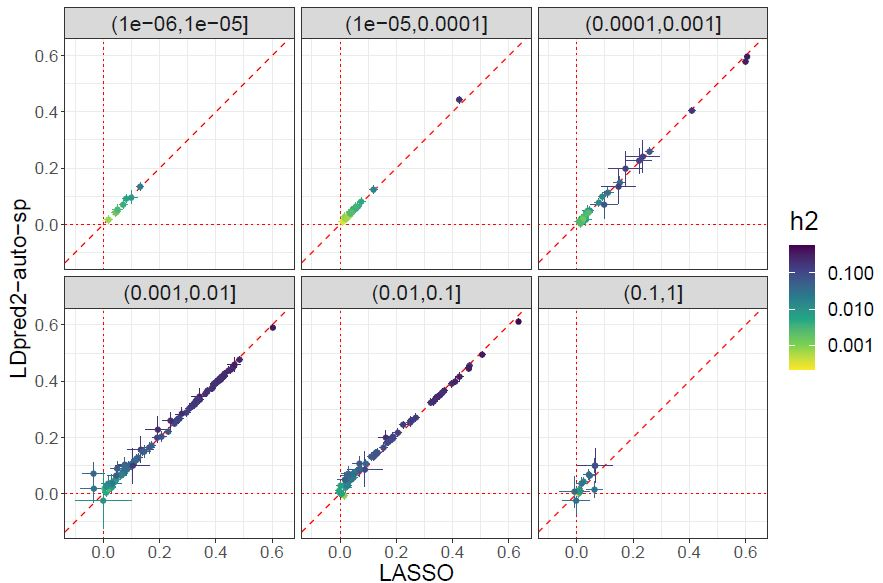
\includegraphics[width=0.9\textwidth]{PLR-ldpred2}
	\caption{\textbf{A)} Partial correlations (and 95\% CI) achieved per phenotype (each point) and per ancestry group (each facet) when training either with LASSO or with LDpred2-auto. \textbf{B)} Focus on the UK facet in A), facetting per proportion of causal variants $p$ and coloring by SNP heritability $h^2$ (estimates from LDpred2-auto).}
	\label{fig:plr-ldpred2}
\end{figure}

\begin{figure}[h]
\centering
\includegraphics[width=0.9\textwidth]{sparse-ldpred2}
\caption{Partial correlations achieved per phenotype (each point) and per ancestry group (each facet) when training either with LDpred2-auto or with LDpred2-auto-sparse (sparse option enabled).}
\label{fig:sparse-ldpred2}
\end{figure}

\begin{figure}[h]
	\centering
	\includegraphics[width=0.8\textwidth]{sparsity-plr}
	\caption{Proportion of variants with non-zero effects in the penalized regression models for each phenotype (point) versus the proportion of causal variants $p$ estimated from LDpred2-auto, colored by the partial correlation achieved in the UK test set.}
	\label{fig:sparsity-plr}
\end{figure}

\begin{figure}[h]
	\centering
	\includegraphics[width=0.8\textwidth]{sparsity-ldpred2}
	\caption{Proportion of variants with non-zero effects in LDpred2-auto-sparse for each phenotype (point) versus the proportion of causal variants $p$ estimated from LDpred2-auto, colored by the SNP heritability $h^2$ estimated from LDpred2-auto.}
	\label{fig:sparsity-ldpred2}
\end{figure}

%%%%%%%%%%%%%%%%%%%%%%%%%%%%%%%%%%%%%%%%%%%%%%%%%%%%%%%%%%%%%%%%%%%%%%%%%%%%%%%%

\begin{figure}[h]
	\centering
	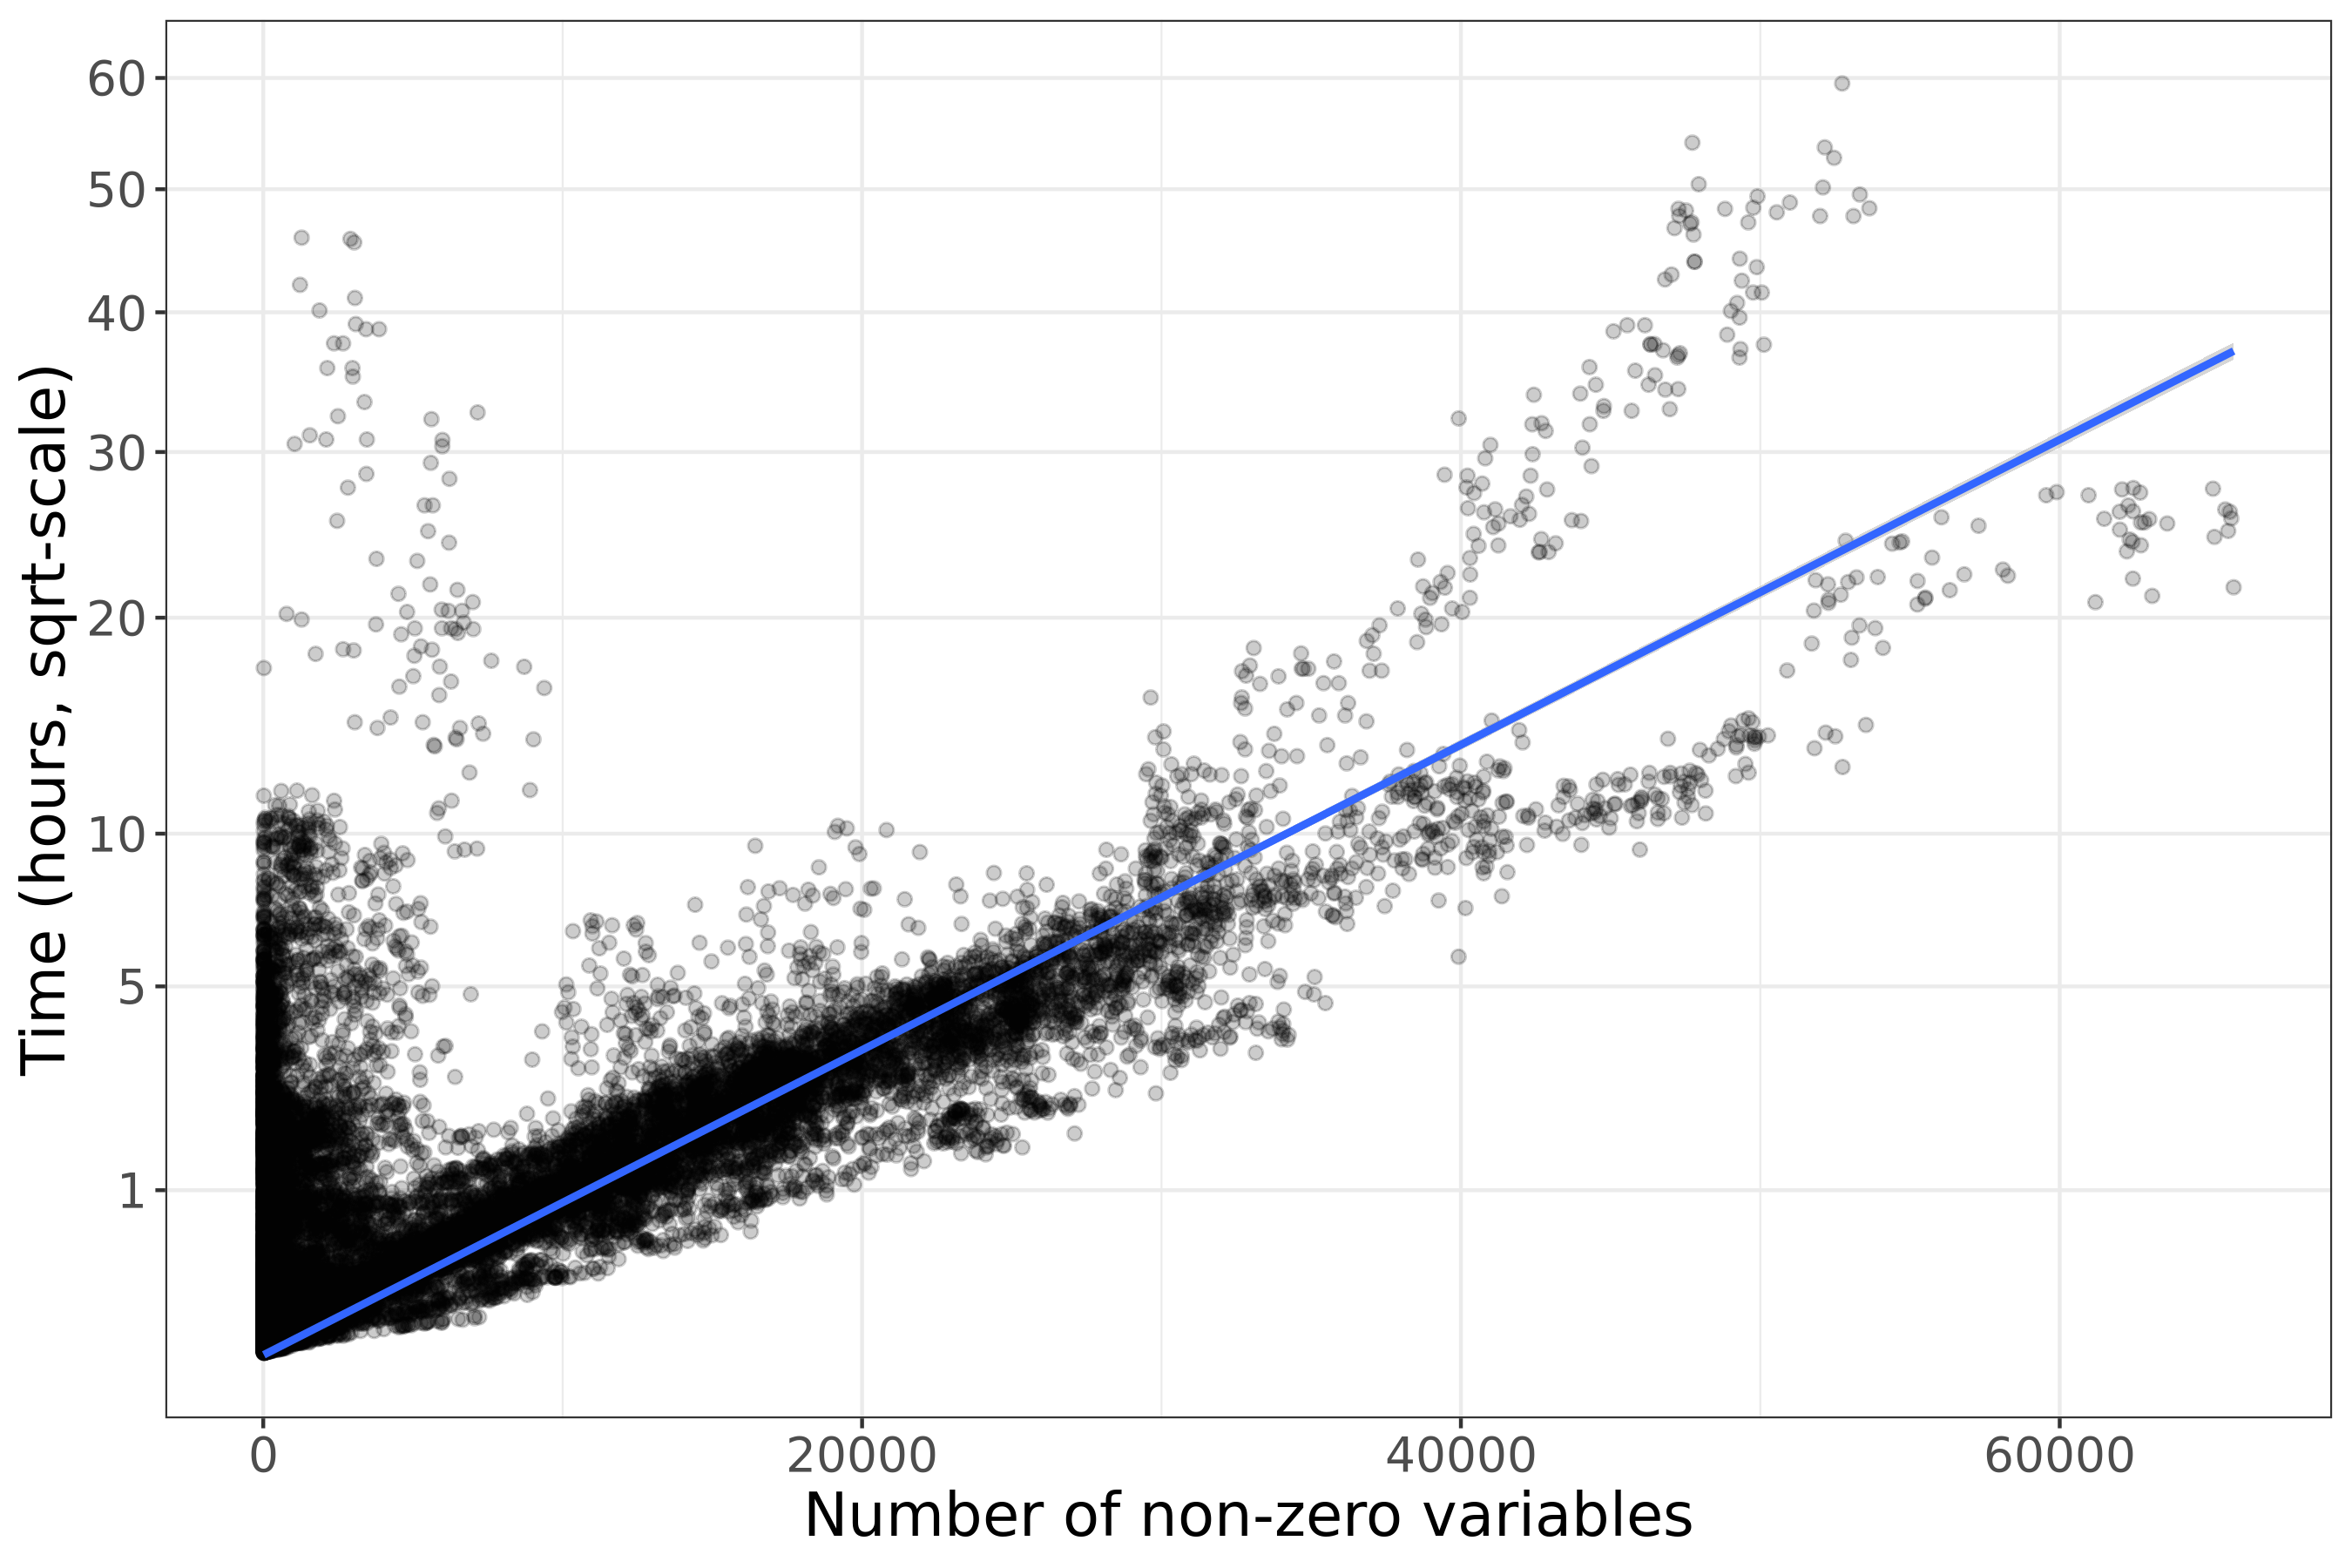
\includegraphics[width=0.9\textwidth]{timings}
	\caption{Computation times for all penalized regression models run using the 1M HapMap3 variants. We recall that we usually run 90 models for each phenotype because we use 9 sets of hyper-parameters and K=10 folds. Computation time is largely quadratic with the number of non-zero effects in the model. It is also dependent on the compute node and the loading of the HPC cluster at the time of running (Figure \ref{fig:timings-ldpred2}).}
	\label{fig:timings-plr}
\end{figure}

\begin{figure}[h]
	\centering
	\includegraphics[width=0.9\textwidth]{timings-ldpred2}
	\caption{Computation times for fitting LDpred2-auto (with default 1000 burn-in iterations + 500 more + sparse option running 150 more) using the 1M HapMap3 variants. Running times should be the same for all phenotypes, yet we see some variability depending on the node used. Some fitting had to be run again because it exceeded the 12-hour timeout, which happened a few times when and the HPC cluster was particularly crowded.}
	\label{fig:timings-ldpred2}
\end{figure}

%%%%%%%%%%%%%%%%%%%%%%%%%%%%%%%%%%%%%%%%%%%%%%%%%%%%%%%%%%%%%%%%%%%%%%%%%%%%%%%%

\begin{figure}[htbp]
	\centerline{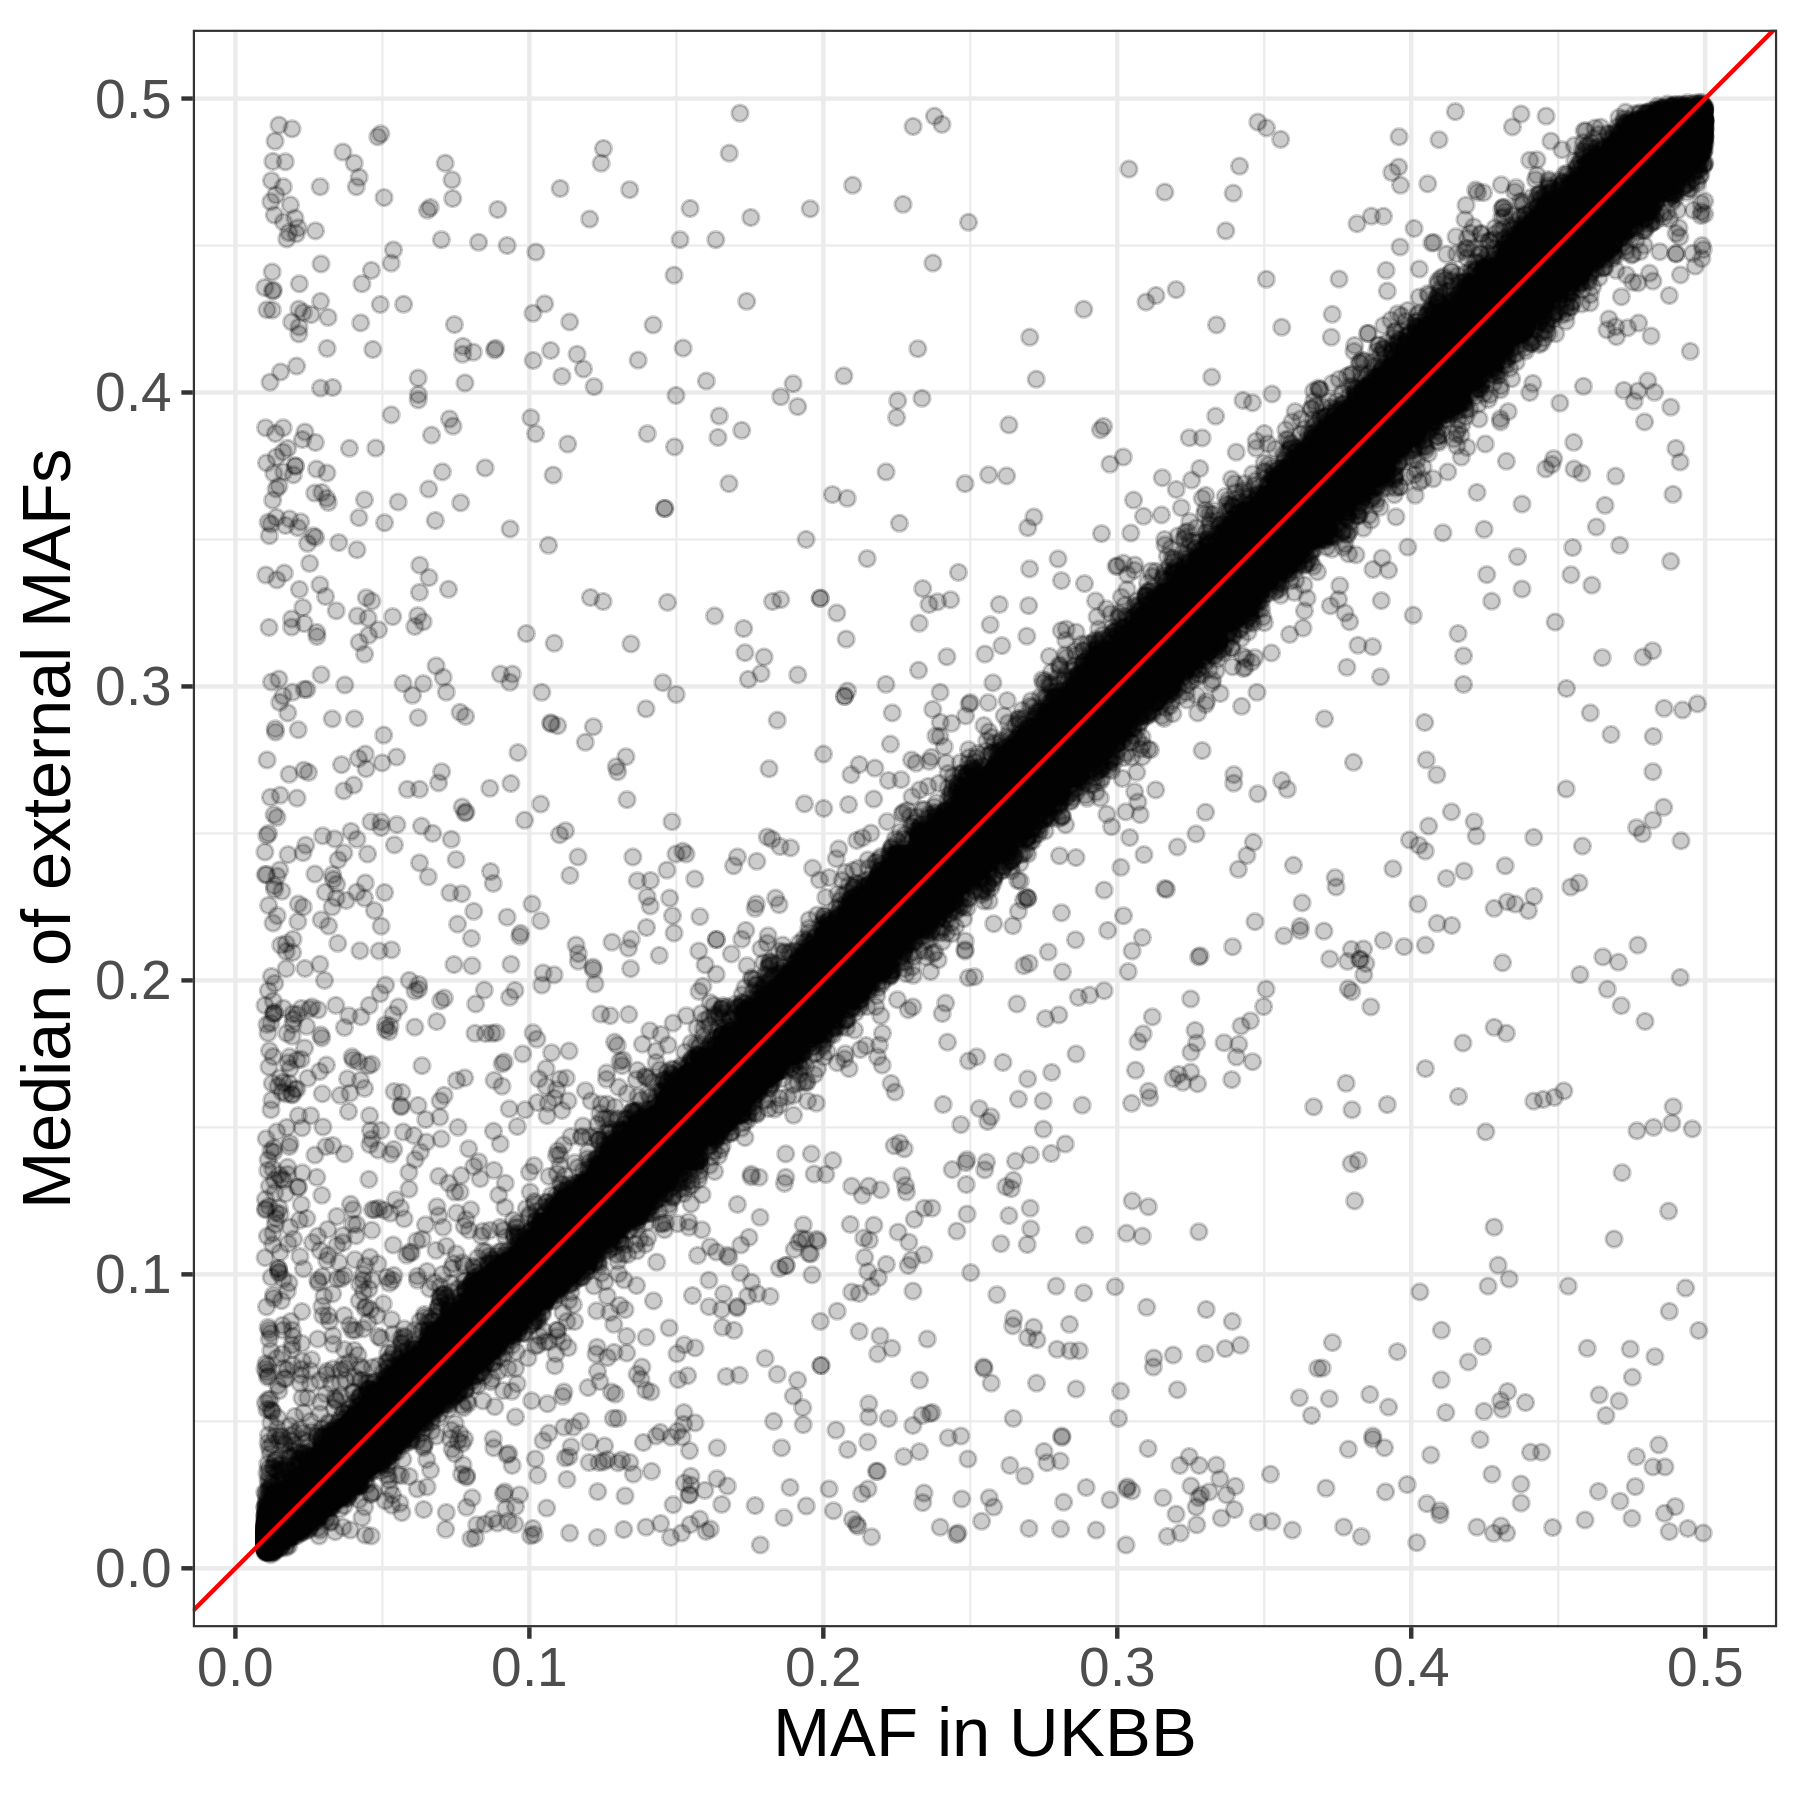
\includegraphics[width=0.85\textwidth]{compare-MAF}}
	\caption{Comparison between frequencies in the UK Biobank and frequencies in external data.}
	\label{fig:compare-MAF}
\end{figure}

\begin{figure}[htbp]
	\centerline{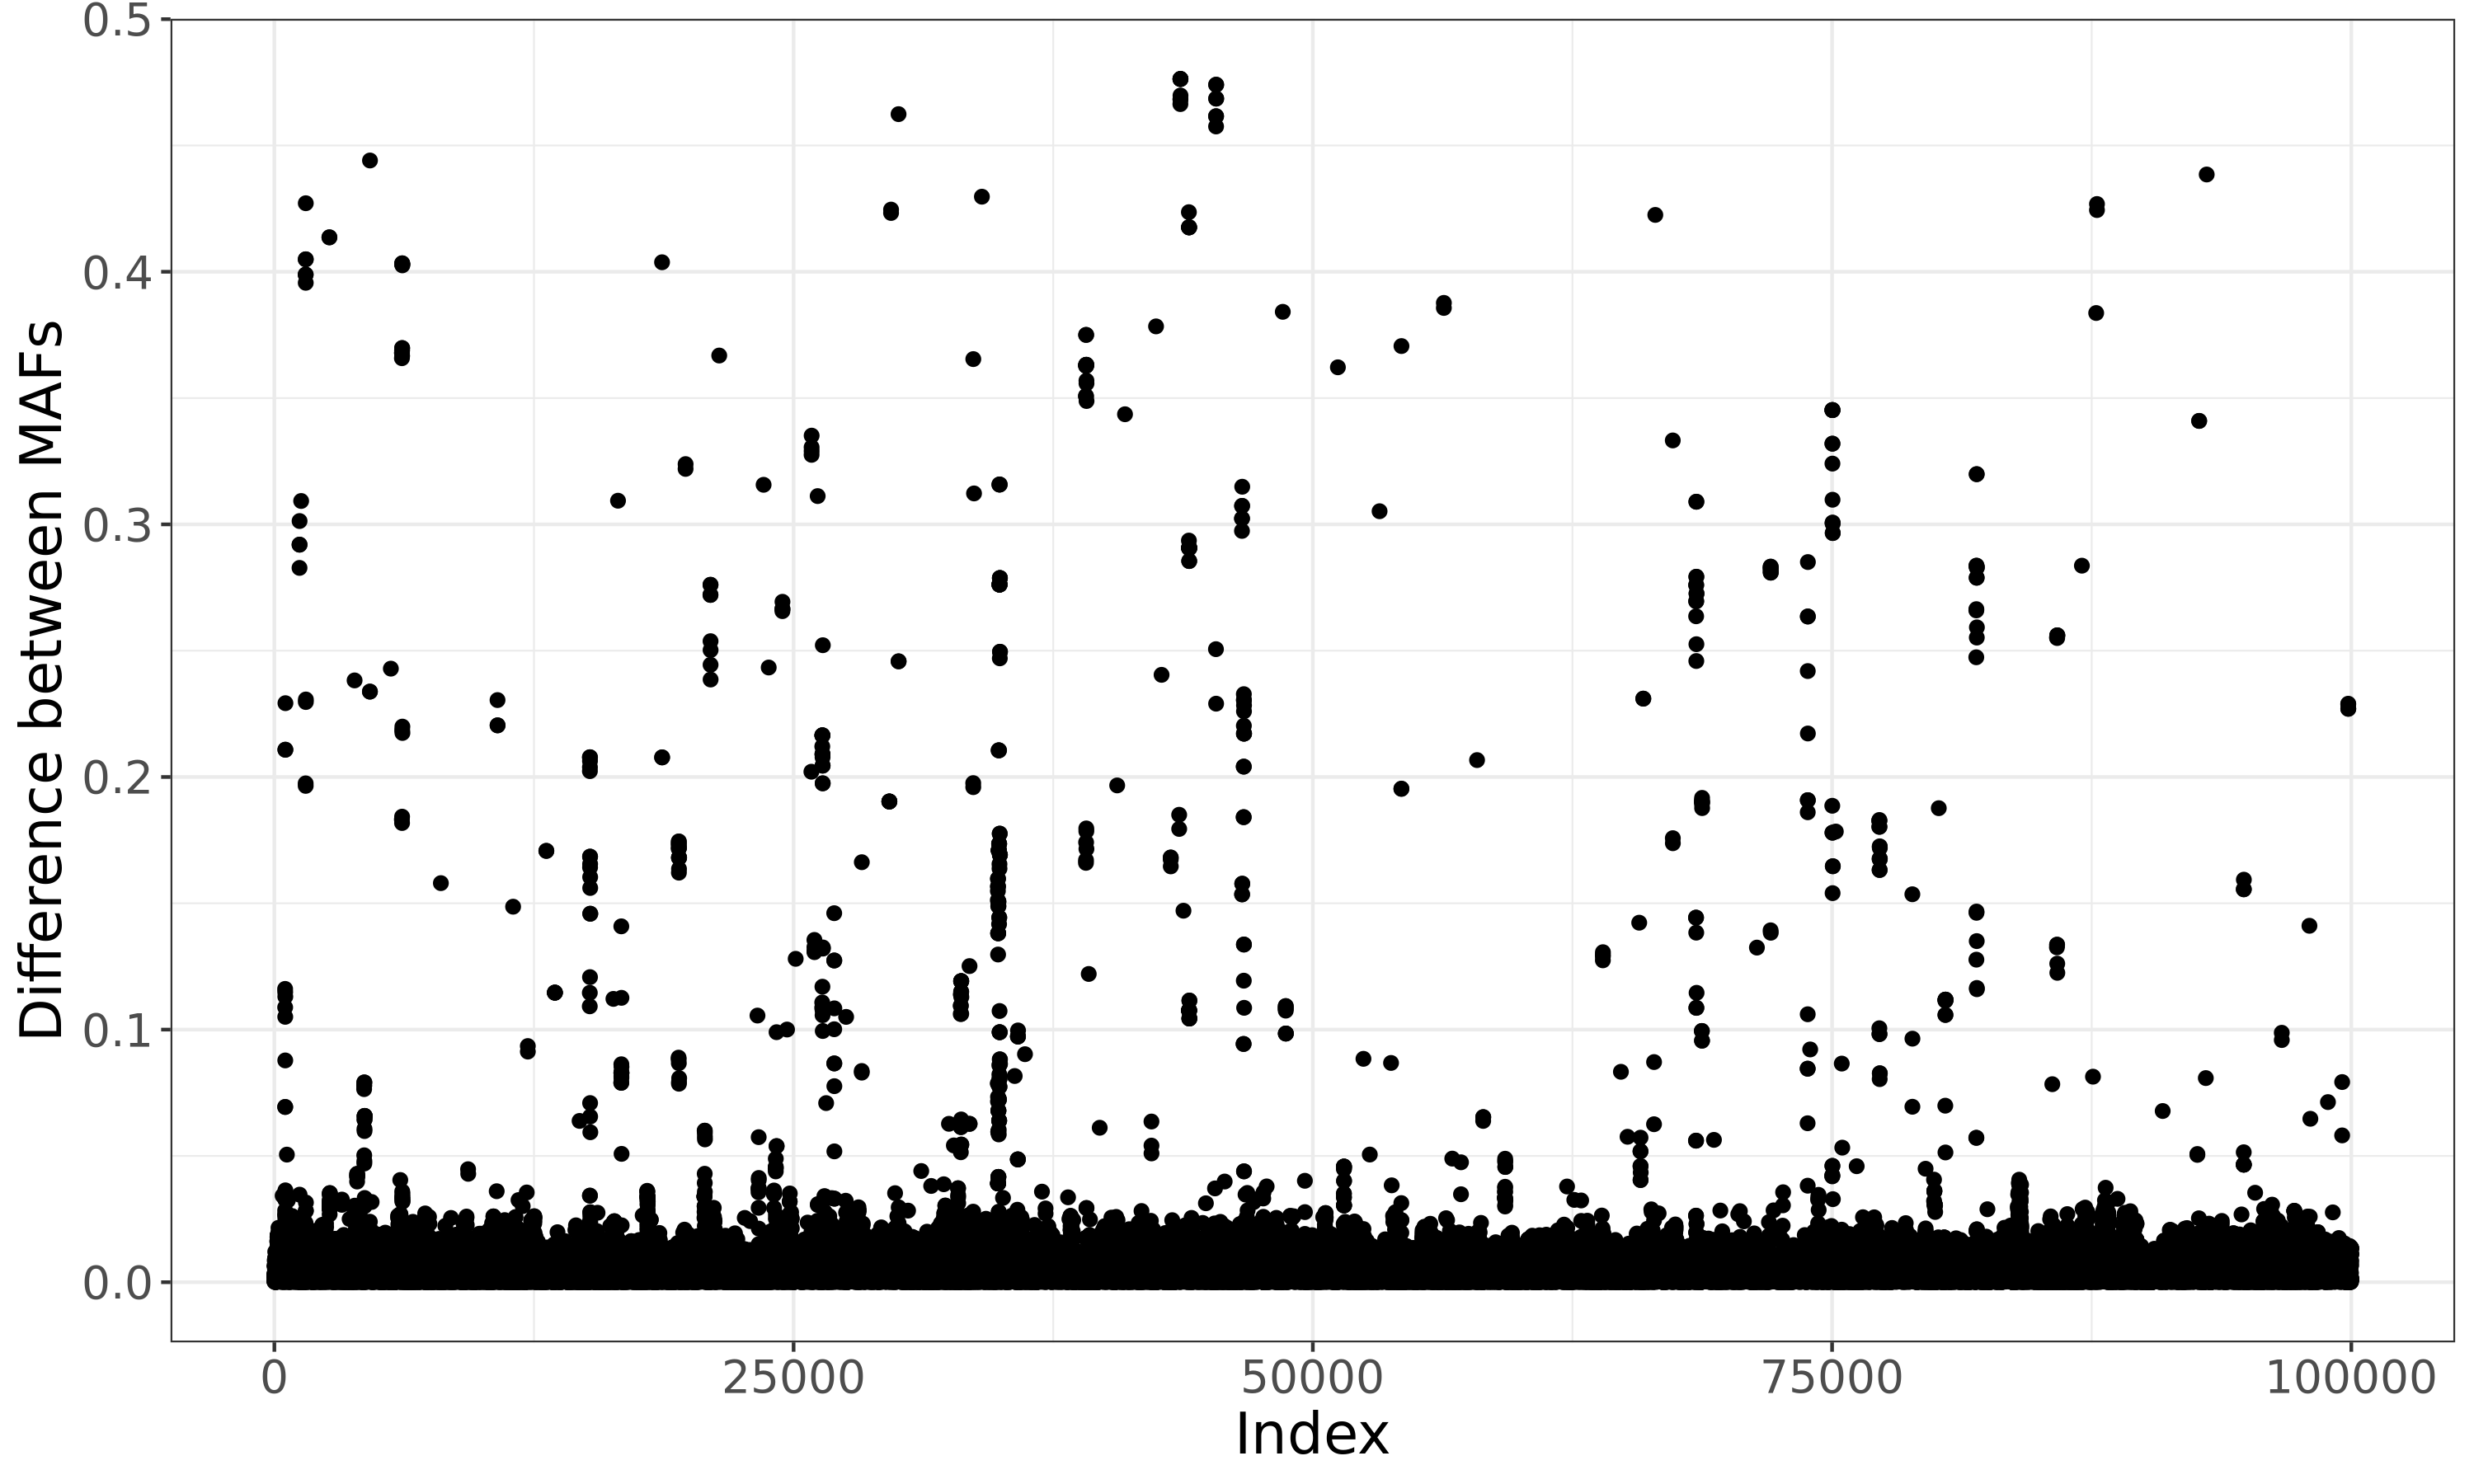
\includegraphics[width=0.95\textwidth]{diff-MAF}}
	\caption{Differences in MAF between the first 100,000 variants in UK Biobank and external data. These differences (likely errors in UKBB) are hypothetically grouped around errors in the genotyped data that propagated to the imputed data.}
	\label{fig:diff-MAF}
\end{figure}

%%%%%%%%%%%%%%%%%%%%%%%%%%%%%%%%%%%%%%%%%%%%%%%%%%%%%%%%%%%%%%%%%%%%%%%%%%%%%%%%

\begin{figure}[htbp]
	\centerline{\includegraphics[width=0.9\textwidth]{qc-plot-new-formula}}
	\caption{Comparison of the standard deviations (SD) computed from both genotypes and summary statistics for the 1000 most associated variants with bilirubin concentration. A) uses the previous formula $\text{sd}(\boldsymbol{G_j}) \approx \frac{\text{sd}(\boldsymbol{y})}{\sqrt{n ~ \text{se}(\hat{\gamma}_j)^2}}$ proposed in \cite{prive2020ldpred2} while B) uses the updated formula $\text{sd}(\boldsymbol{G_j}) \approx \frac{\text{sd}(\boldsymbol{y})}{\sqrt{n ~ \text{se}(\hat{\gamma}_j)^2 + \hat{\gamma}_j^2}}$ proposed here, which does one less approximation.
	The slope slightly larger than 1 can be explained by $\text{sd}(\boldsymbol{y}) > \text{sd}(\boldsymbol{\breve{y}})$.}
	\label{fig:new-formula}
\end{figure}

%%%%%%%%%%%%%%%%%%%%%%%%%%%%%%%%%%%%%%%%%%%%%%%%%%%%%%%%%%%%%%%%%%%%%%%%%%%%%%%%

%\clearpage


%%%%%%%%%%%%%%%%%%%%%%%%%%%%%%%%%%%%%%%%%%%%%%%%%%%%%%%%%%%%%%%%%%%%%%%%%%%%%%%%

\FloatBarrier
%\clearpage

\bibliographystyle{natbib}
\bibliography{refs}

\end{document}
